

%--------------------------------------------------
\section{Contexto empresarial}
\label{sec:Contexto-empresarial}

xxxxxxxxxxxxxxxxxxxxx \cite{Keiningham2011}. xxxxxxxxxxxxxxxxxxxxxxxxxxxxxx.


    %--------------------------------------------------
    \subsection{Tema 1}
    xxxxxxxxxxxxxxxxxxxxxxxxxxxxxx \cite{glady2009predicting, du2007size}.
        
    %--------------------------------------------------
    \subsection{Tema 2}
    xxxxxxxxxxxxxxxxx   \cite{Winkelmann1993PoissonLogisticRegression}
    
    %--------------------------------------------------
    \subsection{Tema 3}
    xxxxxxxxxxxxx \cite{glady2009predicting}xxxxxxxxxxxxxxxx
    
    
    

%--------------------------------------------------
\section{Fundamento teórico de ciencia de datos}
\label{sec:Fundamento-teorico}

    %--------------------------------------------------
    \subsection{Modelo xxxx}

    En este trabajo se considera el modelo estándar Poisson--logístico (\emph{pogit}) para datos de conteo con intensidad latente y observabilidad parcial. Para cada unidad de análisis \(i = 1, \ldots, N\), sea \(y_i\) el conteo observado y \(n_i\) un conteo latente no observable que representa el número total de eventos u oportunidades subyacentes. El modelo se especifica jerárquicamente como
    \begin{equation*}
    \begin{aligned}
        (y_i \mid n_i, \theta_i)
        &\stackrel{ind}{\sim}
        \operatorname{Bin}(n_i, \theta_i),
        \\
        (n_i \mid \lambda_i)
        &\stackrel{ind}{\sim}
        \operatorname{Poisson}(E_i \lambda_i),
    \end{aligned}
    \qquad i = 1, \ldots, N,
    \end{equation*}
    donde \(E_i\) corresponde a un \emph{offset} conocido, \(\theta_i \in (0,1)\) denota la probabilidad de que un evento latente sea observado y \(\lambda_i > 0\) representa la intensidad latente del proceso generador de eventos.
    
    La ecuación binomial del primer nivel modela explícitamente la observabilidad parcial del proceso: condicionalmente a \(n_i\), solo una fracción \(\theta_i\) de los eventos potenciales se registra en los datos observados. Por su parte, la ecuación Poisson del segundo nivel captura la heterogeneidad entre unidades de análisis en el número total de eventos latentes.
    
    %--------------------------------------------------
    \subsection{Modelo xxxx}
    
    La Figura~\ref{fig:pogit} presenta una representación gráfica del modelo mediante notación de placas. Los coeficientes de regresión son compartidos por todas las unidades de análisis, mientras que \(n_i\) y \(y_i\) corresponden, respectivamente, a variables latentes y observadas específicas de cada unidad.
    
    \begin{figure}[H]
        \centering
        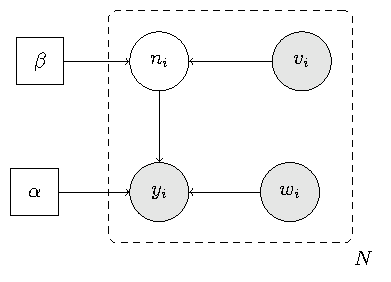
\includegraphics[width=0.5\textwidth]{figuras/modelo_v2.pdf}
        \caption{Representación gráfica del modelo pogit. Los círculos indican variables aleatorias y las flechas indican dependencia condicional. Los nodos sombreados representan cantidades observadas.}
        \label{fig:pogit}
    \end{figure}




















